\chapter{Theoretische Grundlage}
Hier die zugrunde liegenden Grundlagen des Papers.
Quality cuts angeben.

\section{FACT Einleitung}
\begin{wrapfigure}[24]{R}[0pt]{0.5\textwidth}
  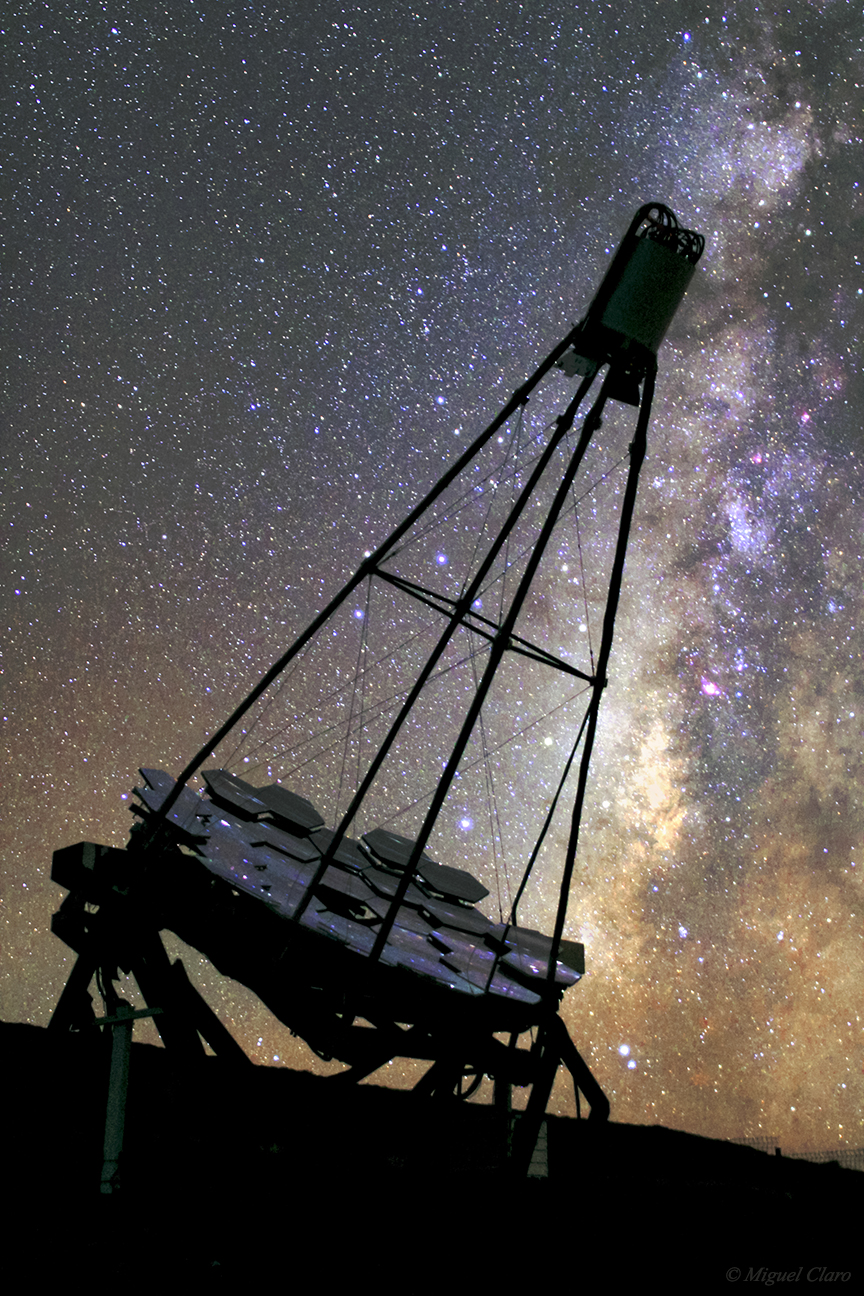
\includegraphics[width=0.5\textwidth]{./logos/FACT.jpg}
  \caption{FACT in Observatiosposition}
  \label{fig:observ}
\end{wrapfigure}
Das FACT (First G-APD Cherenkov Telescope) dient der Überwachung von $\gamma$-Quellen, um bei erhöhter Aktivität, für genauere Observationen größere Telekope zu informieren. Desweiteren erprobt das Telekop die Nutzung von Silizium Photomultiplier (SiMPs) mit welchen es möglich ist, auch an Tagen mit starker diffuser Hintergrundstrahlung Quellen zu observieren. \\

Auf einer höhe von 2200 meter über dem Meeresspiegel befindet sich das Cherenkov Teleskop auf der kanarischen Insel Las Palma. Das Projekt entstand als ein Nachfolgerexperiment des übergebliebenen HEGRA CT3 Telskope, wobei die übergeblieben Spiegel aufbereitet und wiederverwertet werden. (nochmal schöner Formulieren)\\

Die 30 hexongonalen Spiegel bilden eine Gesamtspiegelfläche von \SI{9.51}{\meter\squared} bei einem Blickfeld von \SI{4.5}{\degree}. Die Spiegel sind seid der neuasusrichtung in der Davies-Cotton design ausgerichtet. \cite{??} 
Als erstes Telskope seiner Zeit verwendet FACT SiPMs verwendet anstelle von herkömlichen Photomultiplier Tubes. Halbleiterdetektoren lassen sich mit einer geringerren operation Spannung (< \SI{100}{\volt}) betreiben und sind preiswerter als Photomultiplier, was die Gestaltung des Kameradesigns, als auch die Finanzierung vereinfacht. SiPMs sind aufgrund ihrer hoher Sensitivität dazu in der Laage einzelne Photonen zu detektieren.
Dabei bilden 1440 Kamerapixel das Bild der Kamera, welche jeweils aus einem quadratischen Sensor und einem Plexiglasleiter bestehen. Die einzelne Oberflächen der Hexagonal zulaufenden Plexiglasleiter bilden dabei das Kamerabild.

\section{Entstehung von Cherenkov Schauern}
Trifft ein hochenergetisches Teilchen auf die Atmosphäre löst dieses ein schauer von Sekundärteilchen aus. Dabei ist die Energie der erzeugten Teilchen stets geringer als das einfallende Teilchen. Dabei wird zwischen zwei verschiedenen Arten von Schauern unterschieden. 

\textbf{Møglicher weise Tikz picture}

Trifft ein hochenergetisches $\gamma$-Quant auf die Atmosphaere, so wird es wahrscheinlich im Columbwall der Molekühle durch Paarerzeugung ein Elektronen-Positron-Paar erzeugen. Anschließend kann bei hinreichend großer Energie das Elektron durch Bremsstrahlung weiter Photonen erzeugen. 
\begin{eqnarray}
  \gamma \rightarrow& e^{+} + e^{-} \\
  e^{+} \rightarrow& e^{+'} + \gamma \\
  e^{-} \rightarrow& e^{-'} + \gamma 
\end{eqnarray}
Dieser Prozess ist solange fortlaufend bis die Energie der Teilchen zu klein ist ein neues Teilchenpaar zu erzeugen. Trifft ein geladenes kosmisches Teilchen in die Atmosphäre so kann dieses viele verschiedene Sekundarteilchen bilden. Dabei entstehen unter anderem Neutronen, Protonen und Pionen welche wiederum zerstrahlen. 
\begin{eqnarray}
  \pi^{0} \rightarrow& \gamma + \gamma \\
  \pi^{+} \rightarrow& \mu^{+} + \nu_{\mu} \\
  \pi^{-} \rightarrow& \mu^{-} + \bar{\nu}_{\mu}
\end{eqnarray}
Entseht bei der Paarbildung schon früh ein $\pi^{0}$~Meson, so ist der Teilchenschauer kaum von dem eines $\gamma$-Quanten zu unterscheiden. \newline
Bewegt sich ein Teilchen schneller als die Lichtgeschwindigkeit in dem Medium polarisiert es dieses Kurzzeitig. Dabei wird eine kohärente Schockwelle in Bewegungsrichtung abgestrahlt. Diese Bilden ein Mach-Kegel aus dessen Öffungswinkel $\theta$ von dem Brechungsindex $n$ des Mediums und der Phasengeschwindikeit der Welle abhängt.
\begin{equation}
  \cos  \theta = \frac{1}{\text{n} \beta}
  %  \label{}
\end{equation}

\section{Bildgebene Paramter}
\begin{figure}[H]
  \centering
  \includegraphics[width=0.5\textwidth]{logos/detektor.pdf}
  \caption{Muss noch eine bessere Grafik gesucht werden}
\end{figure}
Fällt ein Schauer in das Teleskop erzeugt dieses in der Kamera ein Bild. Nach dem Artefakte und äußere Einflüsse (noch mehr zu schreiben ?) bereinigt worden sind, wird anhand der Pixel die auf den Tscherenkovschauer zurück zu führen sind, die Hillas Parameter berechnet. Dazu wird im wesentlichen eine Gaußverteilung furch die Helligkeit der Pixel gefittet. Zu den Hillasparameter zählen:
\begin{itemize}
  \item \textbf{width/length:} Hauptachse der Ellipse
  \item \textbf{size:} Anzahl an Pixel im Schauer
  \item \textbf{CoG:} Schwerpunkt des Schauers
  \item \textbf{Core of image:} Helligkeit der einzelnen Pixel
  \item \textbf{DISP:} Abstand zwischen Schwerpunkt des Schauers und der gemessenen Quellposition. Anhand der parameter width und length wird DISP abgeschätzt um die gemessene Quellposition zu ermitteln. Dabei gibt es zwei mögliche Vorzeichen, welche man durch die observation der zeitlichen Konzentration der einzelenen Pixel im Schauer abzuschätzen versucht.
  \item \textbf{Source Position:} erwatete Quellposition
  \item \textbf{$\theta$:} Winkelzwischen der gemessenen und echten Quellposition
\end{itemize}
\section{Wobble Observation Strategy}
\begin{wrapfigure}[18]{L}[0pt]{0.53\textwidth}
  \includegraphics[width=0.5\textwidth]{logos/wobble.pdf}
  \caption{Wobble observation muss noch zitiert werden. Theme dissertaion}
\end{wrapfigure}
Die Wobble Observation Strategy zeichnet aus, dass im gegensatz zur klassischen Methode nicht hintereinander On/Off postion beobachtet werden. Stattdessen wird die erwartete Quellpostion \SI{0.6}{\degree} neben die Kameraachse gelegt. Dies hatt zur Folge dass es mehrere Positionen mit dem selben offest und symmetrie gibt. Bei der standard analyse bei Fact koennen so neben der ON-Position, f↓nf Off-Positionen mit demselben Kippungswinkel zur Kameraachse gemessen. Somit ergibt sich fuer jedes Datensample jeweils ein $\theta_\text{on}$ und fuenf $\theta_\text{off}$. Fuer kleine $\theta$ Winkel kann geschlossen werden, dass das gemessene Teilchen aus richtung der Quelle kam und vermutlich ein $\gamma$-Quant ist. Da der Hadron untergrund isotrop in alle Richtungen auftritt, sollten bei Hadronischen Schauern eine Thetaverteilung in etwa gleichverteilt seien  Zu den Vorteilen dieser Methode zaehlen das keine Extra OFF Daten genommen werden muessen. Somit ist es moeglich die Messzeit der Quellaktivitaet zu maximieren. Desweiteren kann durch die gleichzeitige Daten nahme davon ausgegangen werden das fuer die ON/OFF-Positionen annaehernd die selben Wetterbedingungen gelten. 

\section{Überwachtes Maschinelles Lernen}
Zur Auswertung der Datenmengen von 300 GB bis 1 TB cite MaxNoethe die FACT jede Nacht aufnimmt werden maschinelle lernmethodenen verwendet. Maschinelles lernen kann dazu genutzt werden Muster und Strukturen auf Datensaetze zu erkennen und zukuenftige ereignisse hervorzusagen. Dabei wird zwischen ueberwachtem und unueberwachtem Training unterschieden. Unueberwachtes lernen kennzeichnet sich dadurch, dass versucht wird auf dem Trainingsdatensatz $X$ spannende Muster zu erkennen.  Ziel des Ueberwachten lernens ist es bei einem gegebenen Trainingsset welches aus Input variablen $X$ und Zielvariablen $y$ besteht Modelle zu finden, welche $X$ bestmoeglich auf $y$ abbilden. \newline
Zunachst muss dafur das Modell auf einen Datensatz trainiert werden. Daf↓r wird der Datensatz ($X$, $y$) in zwei teile aufgeteilt, dem Trainings- und dem Testdatensatz. Dabei wird das Modell auf den Trainingsdatensatz optimiert und anschließend auf dem Testdatensatz evaluiert. Dabei ist darauf zu achten, dass das Modell nicht nur den Trainingsdatensatz auswendig lernt (uebertraining), sondern allgemein genug bleibt auch aehnliche Datensaetze genau vorherzusagen. Dies geschieht durch beschraenkung der Modelle.

\subsection{Entscheidungsbaum}
\begin{wrapfigure}[14]{R}[0pt]{0.5\textwidth}
  \centering
  \includegraphics[width=0.5\textwidth]{logos/tikz/tree/tree.pdf}
  \caption{Entscheidungsbaum der Tiefe 2 bei Gamma Handron Seperation}
\end{wrapfigure}
Ziel eines ein Modell zu entwickeln, welches anhand eines Trainingsdatensatzes die eingangsvariablen $x$ auf die Zielvariablen $Y$ abbildet. Daf↓r werden eine Verkettung von Entscheidungen durchgefuehrt,  
confidence scores
\subsection{Random Forest}

\subsection{extra boosted Decisiontree}

\section{Evaluieren}

\subsection{Li und Ma Signifikanz}

\begin{equation}
S = \sqrt{2} \left( N_\text{on} \ln \left[ \frac{1+ \alpha}{\alpha}\left( \frac{N_\text{on}}{N_\text{on} + N_\text{off}} \right) \right] + N_\text{off} \ln \left[ \left( 1+ \alpha \right) \left( \frac{N_\text{off}}{N_\text{on} + N_\text{off}} \right) \right] \right)^{1/2}
\end{equation}
\subsection{Receiver Operating Characteristic}

